\documentclass[12pt,fleqn]{article}\usepackage{../../common}
\begin{document}
Ders 2

Karakteristik Eğriler Metodu

Bu metot katsayıları sabit olmayan 1. derece, lineer PDE çözmemize yardım
eder. PDE şu formdadır

$$ \frac{\partial u}{\partial x} + 
p(x,y) \frac{\partial u}{\partial y} = 0 
\mlabel{1}
 $$

ve $p(x,y)$, $x,y$ değişkenlerinin bir fonksiyonudur. 

Üstteki denklemi iki vektörün noktasal çarpımı olarak ta görebiliriz. 

$$ 
<\frac{\partial u}{\partial x}, \frac{\partial u}{\partial y}> \cdot 
<1,p(x,y)> = 0
 $$

Bu açıdan bakınca yukarıdaki ifade yeni bir şey söylüyor, $u$'nun
$<1,p(x,y)>$ vektörüne göre yönsel türevinin sıfır olduğunu söylüyor, yani
o yönde hiçbir değişim yok. 

Şimdi tek başına $<1,p(x,y)>$ vektörünü düşünelim, her değişik $x,y$ için
bu vektörler bir vektör alanı oluşturur, bu alandaki vektörleri bir eğrinin
``belli bir noktadaki eğimini gösterdiği'' şeklinde alabiliriz. O
noktalardaki eğim $p(x,y) / 1$ olacaktır doğal olarak, o zaman bu eğriler
için şöyle bir basit diferansiyel denklem (ODE) yazabiliriz.

$$ \frac{dy}{dx} = \frac{p(x,y)}{1} $$

ya da

$$ \frac{dy}{dx} = p(x,y) 
\mlabel{2}
$$

Bu ODE bir yön alanı (direction field) oluşturur, bkz [1].

Şimdi geri adım atıp her şeye tekrar bakalım. (1) diyor ki $x,y$ noktasında
$u$'nun $<1,p(x,y)>$ yönündeki yönsel türevi sıfır. Yani $x,y$ noktasında
$<1,p(x,y)>$ yönünde ilerlersek $u$ hiç değişmeyecek. 

Aynı zamanda $<1,p(x,y)>$ vektörleri (2) için bir yönsel alan da
tanımlıyor!  Bilindiği gibi (2) denklemi çözüm eğrileri (solution curves)
ortaya çıkartır, ve ne raslantı ki (!) bu çözüm eğrilerinin her birinde
(1)'deki $u$ sabit kalır. 

Örnek 

$$ \frac{\partial u}{\partial x} + 
x \frac{\partial u}{\partial y} = 0 
 $$

Yani $p(x,y) = x$. O zaman 

$$ \frac{dy}{dx} = x $$

denklemini çözeriz, ve 

$$ y = \frac{1}{2}x^2 + C $$

karakteristik eğrilerini elde ederiz. Tekrar düzenlersek

$$ y - \frac{1}{2}x^2 = C $$

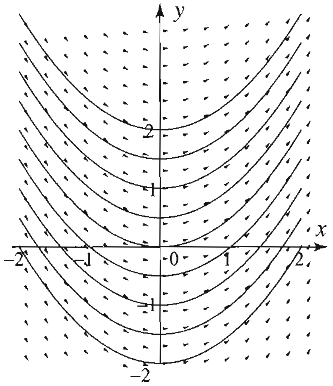
\includegraphics[height=4cm]{2_1.png}

O zaman PDE'nin genel çözümü 

$$ u(x,y) = f(C) = f(y - \frac{1}{2}x^2) $$

diyebiliriz, $f$ rasgele bir fonksiyondur, söylenmeye uğraşılan farklı
sabitlere tekabül eden $u$'lardır. PDE çözümü $u$'nun sabite eşit olmasıyla
alakalı çünkü PDE'yi yönsel türev olarak temsil edince bu sonuca
varıyoruz. Üstteki denklem de karakteristik eğriler açısından gelerek o
sabiti bize sağlıyor.

$f$'in genel çözüm olduğunu ana denklemde yerine koyarak test edebiliriz.

Örnek 

$$ u_x + yu_y = 0 $$

O zaman 

$$ \frac{dy}{dx} = y $$

$$ y = Ce^x $$

ya da

$$  C = e^{-x}y$$

Genel çözüm 

$$ u(x,y) = f(C) = f(e^{-x}y) $$

PDE içinde yerine koyarak sonucu kontrol edelim

$$ u_x + yu_y = 
-f'(e^{-x}y)e^{-x}y + y f'(e^{-x}y) e^{-x} = 0
 $$

Dalga Denklemi 

$$ u_{tt} = c^2 u_{xx} $$

dalga denklemi olarak bilinir. Bir diğer şekilde 

$$ u_{tt} - c^2 u_{xx} = 0$$

Bu denklemi operatörlerin faktorize edilmiş hali olarak görmek mümkündür. 

$$ u_{tt} - c^2 u_{xx} = 
\bigg( \frac{\partial }{\partial t} - c \frac{\partial }{\partial x} \bigg)
\bigg( \frac{\partial }{\partial t} + c \frac{\partial }{\partial x} \bigg)
u = 0
\mlabel{3}
$$

Eşitliğin sağ tarafındaki operatörler hakikaten dalga denklemine tekabül
ediyor mu? Kontrol edelim, üstteki $u$ üzerinde etki eden ilk operatör şu
şekilde açılıyor

$$ \bigg( \frac{\partial }{\partial t} + c \frac{\partial }{\partial x}
\bigg) u = 
\frac{\partial u}{\partial t} + c \frac{\partial u}{\partial x}
$$

Şimdi ikinci operatörü uygulayalım (bu sefer eksi olan operatör), yani şunu
hesaplayalım, ve üstteki eşitliğin sağ tarafı şöyle olur

$$ 
\bigg( \frac{\partial }{\partial t} - c \frac{\partial }{\partial x} \bigg)
\frac{\partial u}{\partial t} + c \frac{\partial u}{\partial x} 
 $$

$$ = 
\frac{\partial ^2 u}{\partial t^2} + 
c \frac{\partial u}{\partial x \partial t} - 
c \frac{\partial u}{\partial t \partial x} - 
c^2\frac{\partial ^2 u}{\partial x^2} 
 $$

$u_{xt} = u_{tx}$ olduğuna göre ortadaki iki terim iptal olur

$$ = 
\frac{\partial ^2 u}{\partial t^2} -
c^2\frac{\partial ^2 u}{\partial x^2} 
 $$

Açılımı ispatlamış olduk. 

Çözümü bulalım. Karakteristik kordinat (characteristic coordinate)
yöntemini kullanalım. Bu sefer ilginç bir şey yapacağız, kordinat
değişimini tanımlayan eşitliklerden sonra operatörler üzerinde sanki
cebirsel büyüklüklermiş gibi işlem yapacağız. 

$$ \xi = x + ct $$

$$ \eta = x - ct $$

Bu kordinat değişimi için bir tahmin yürüttük. Doğru olup olmadığını şimdi
göreceğiz. 

$$ \partial_x = \partial_\xi + \partial_\eta $$

$$ \partial_t = c\partial_\xi - c \partial_\eta $$

Bu formüller aslında 1. derste gördüğümüz (1),(2) formüllerine benziyor,
sadece üsttekiler pür operatör formunda ve sabitler bu probleme göre
ayarlı. 

Şimdi iki üstteki formülü $c$ ile çarpıp bir üstteki formül ile toplarsak,
sonuç 

$$ \partial_t + c\partial_x = 2c \partial_\xi $$

Toplamak yerine bir üstteki formülden iki üstteki formülü çıkartırsak

$$ \partial_t - c\partial_x = -2c \partial_\eta $$

Üstteki eşitliklerin sol tarafları, daha önce PDE için operatör açılımı
yaptığımızda ortaya çıkan operatörler ile aynı. O zaman açılımda yerlerine
koyarsak, PDE şöyle olur

$$ (2c\partial_\xi)(-2c\partial_\eta)u = 0 $$

Diğer bir deyişle 

$$ u_{\xi_\eta} = 0 $$

Biliyoruz ki $c \ne 0$. Bu transform edilmiş denklemin çözümü nedir? İlk
önce $\eta$'ya göre entegral alırız, 

$$ u_\xi = f(\xi) $$

Bir daha entegral alırız

$$ u = F(\xi) + G(\eta) $$

ki $F' = f$ olarak alındı. Burada aslında $f,F$'in ne oldukları pek önemli
değil, ikisi de rasgele fonksiyonlar, tek önemli olan aldıkları
parametreler. O zaman çözüm 

$$ u(x,t) = F(x+ct) + G(x-ct) $$

ki $F,G$ rasgele fonksiyonlar. 

Kaynaklar

[1] Bayramli, Diferansiyel  Denklemler, {\em Ders 1}

\end{document}
